\documentclass[11pt]{article}

\usepackage[a4paper,margin=0.75in]{geometry}
\usepackage{amsmath,amssymb}
\usepackage{graphicx}
\usepackage{booktabs}
\usepackage{array}
\usepackage{float}
\usepackage{hyperref}
\usepackage{enumitem}
\usepackage{xcolor}
\usepackage{tikz}
\usetikzlibrary{positioning,arrows.meta,shapes.geometric}

\setlist{nosep}
\renewcommand{\arraystretch}{1.3}

\tikzset{
layer/.style={
draw,
rounded corners,
minimum width=2.2cm,
minimum height=0.9cm,
align=center,
fill=blue!10
},
arrow/.style={
-{Latex[length=3mm]},
thick
}
}

\begin{document}

%%%%%%%%%%%%%%%%%%%%%%%%%%%%%%%%%%%%%%%%%%%%%%%%%%%%%%%%%%%%

\begin{center}

{\Large\textbf{Shiv Nadar University Chennai}}

\vspace{3mm}

{\large\textbf{CS3807 -- Deep Learning Laboratory}}

\vspace{3mm}

{\Large\textbf{Experiment 4}}

\vspace{2mm}

{\Large\textbf{Comparative Study of Deep Convolutional Neural}}

{\Large\textbf{Network Architectures Using Transfer Learning}}
\textbf{Repository Link:}
\textbf{\url{https://github.com/Atharsh2910/Deep_Learning_Lab/tree/main/Lab4}
}
\end{center}

\vspace{5mm}

\begin{tabular}{|p{3.8cm}|p{8cm}|p{2cm}|}
\hline
Degree \& Branch & B.Tech Artificial Intelligence \& Data Science & Semester V\\ \hline
Subject Code \& Name & CS3807 -- Deep Learning Laboratory & AY: 2026--27\\ \hline
\end{tabular}

\begin{tabular}{|p{3.5cm}|p{8cm}|}
\hline
\textbf{Name} & {ATHARSH S U}\\ \hline
\textbf{Register Number} &{24011101008} \\ \hline
\textbf{Roll Number} &{24110049} \\ \hline
\textbf{Class} & {AI-DS 'A'}\\ \hline
\end{tabular}
\vspace{3mm}

%%%%%%%%%%%%%%%%%%%%%%%%%%%%%%%%%%%%%%%%%%%%%%%%%%%%%%%%%%%%

\section*{1. Objective}

The objectives of this experiment are

\begin{itemize}

\item Study the evolution of deep CNN architectures.

\item Compare LeNet-5, AlexNet, VGG16, GoogleNet and ResNet.

\item Understand transfer learning.

\item Fine tune pretrained CNN models.

\item Compare classification performance of different architectures.

\end{itemize}

%%%%%%%%%%%%%%%%%%%%%%%%%%%%%%%%%%%%%%%%%%%%%%%%%%%%%%%%%%%%

\section*{2. Learning Outcomes}

After completing this experiment students will be able to

\begin{enumerate}

\item Explain modern CNN architectures.

\item Differentiate LeNet, AlexNet, VGG16, GoogleNet and ResNet.

\item Implement transfer learning.

\item Fine tune pretrained CNN models.

\item Compare CNN architectures using performance metrics.

\end{enumerate}

%%%%%%%%%%%%%%%%%%%%%%%%%%%%%%%%%%%%%%%%%%%%%%%%%%%%%%%%%%%%

\section*{3. Introduction}

Deep Convolutional Neural Networks have become the dominant models for
computer vision applications because they automatically learn hierarchical
features from images. The evolution of CNNs has focused on improving
classification accuracy while reducing computational complexity and
training difficulties.

The progression of CNN architectures began with LeNet-5 and has evolved
through AlexNet, VGGNet, GoogleNet, and ResNet. Each architecture
introduced important innovations that significantly improved image
classification performance.

%%%%%%%%%%%%%%%%%%%%%%%%%%%%%%%%%%%%%%%%%%%%%%%%%%%%%%%%%%%%

\section*{4. Evolution of CNN Architectures}

\begin{center}

\begin{tabular}{|c|c|p{7cm}|}

\hline

Model & Year & Major Contribution\\

\hline

LeNet-5 & 1998 &
First practical convolutional neural network\\

\hline

AlexNet & 2012 &
ReLU activation, Dropout and GPU training\\

\hline

VGG16 & 2014 &
Uniform $3\times3$ convolution filters\\

\hline

GoogleNet & 2014 &
Inception modules for multi-scale feature extraction\\

\hline

ResNet & 2015 &
Residual learning using skip connections\\

\hline

\end{tabular}

\end{center}

%%%%%%%%%%%%%%%%%%%%%%%%%%%%%%%%%%%%%%%%%%%%%%%%%%%%%%%%%%%%

\section*{5. LeNet-5}

LeNet-5 was proposed by Yann LeCun in 1998 for handwritten digit
recognition. It consists of two convolution layers, two average pooling
layers and fully connected layers. It demonstrated that convolutional
networks could automatically learn image features without handcrafted
feature extraction.


Advantages

\begin{itemize}

\item Small number of parameters

\item Fast training

\item Suitable for OCR

\end{itemize}

%%%%%%%%%%%%%%%%%%%%%%%%%%%%%%%%%%%%%%%%%%%%%%%%%%%%%%%%%%%%

\section*{6. AlexNet}

AlexNet won the ImageNet Challenge in 2012 by reducing the
classification error significantly. It introduced ReLU activation,
Dropout regularization and GPU training.


Major innovations

\begin{itemize}

\item ReLU activation

\item Dropout

\item GPU implementation

\item Data augmentation

\end{itemize}

%%%%%%%%%%%%%%%%%%%%%%%%%%%%%%%%%%%%%%%%%%%%%%%%%%%%%%%%%%%%

\section*{7. VGG16}

VGG16 demonstrated that using multiple small $3\times3$ convolution
filters could outperform larger filters while increasing network depth.


Advantages

\begin{itemize}

\item Excellent feature extraction

\item Simple architecture

\item High classification accuracy

\end{itemize}

%%%%%%%%%%%%%%%%%%%%%%%%%%%%%%%%%%%%%%%%%%%%%%%%%%%%%%%%%%%%

\section*{8. Comparison of Architectures}

\begin{center}

\begin{tabular}{|l|c|c|c|}

\hline

Architecture &
Depth &
Parameters &
Main Contribution\\

\hline

LeNet-5 &
7 &
60K &
First CNN\\

AlexNet &
8 &
61M &
ReLU + Dropout\\

VGG16 &
16 &
138M &
Deep 3$\times3$ filters\\

GoogleNet &
22 &
6.8M &
Inception Modules\\

ResNet50 &
50 &
25.6M &
Residual Learning\\

\hline

\end{tabular}

\end{center}

% --------- CONTINUE WITH PART 2 ---------
%%%%%%%%%%%%%%%%%%%%%%%%%%%%%%%%%%%%%%%%%%%%%%%%%%%%%%%%%%%%
\section*{9. GoogleNet (Inception Network)}

GoogleNet, proposed by Szegedy \textit{et al.} in 2014, introduced the
\textbf{Inception Module}, which performs multiple convolution operations
in parallel using different filter sizes. Instead of using only a single
kernel size, GoogleNet simultaneously applies $1\times1$, $3\times3$,
$5\times5$ convolutions and max pooling. The outputs are concatenated to
obtain multi-scale feature representations.

The use of $1\times1$ convolutions before larger kernels reduces the
number of trainable parameters and computational complexity.


Advantages

\begin{itemize}
\item Multi-scale feature extraction.
\item Fewer parameters than VGG16.
\item High computational efficiency.
\item Better classification performance.
\end{itemize}

%%%%%%%%%%%%%%%%%%%%%%%%%%%%%%%%%%%%%%%%%%%%%%%%%%%%%%%%%%%%

\section*{10. ResNet}

Increasing CNN depth often causes the \textbf{vanishing gradient problem},
making optimization difficult. ResNet solves this issue using
\textbf{skip (residual) connections}, allowing gradients to flow directly
through the network.

Instead of learning

\[
H(x)
\]

ResNet learns

\[
F(x)=H(x)-x
\]

thus,

\[
Output = F(x)+x
\]

where

\begin{itemize}
\item $F(x)$ = Residual Mapping
\item $x$ = Identity Mapping
\end{itemize}

\begin{figure}[H]
\centering

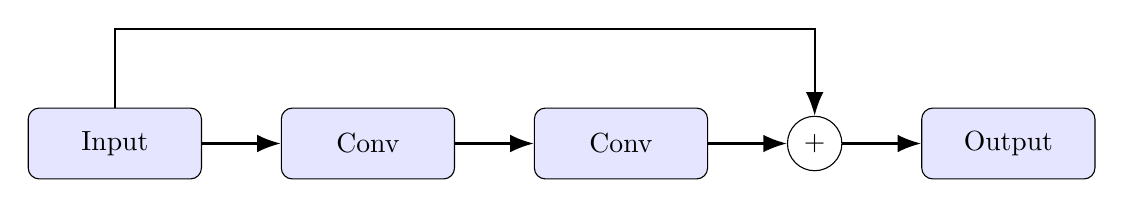
\begin{tikzpicture}[node distance=1cm]

\node[layer](input){Input};

\node[layer,right=of input](conv1){Conv};

\node[layer,right=of conv1](conv2){Conv};

\node[circle,draw,right=of conv2](add){+};

\node[layer,right=of add](output){Output};

\draw[arrow](input)--(conv1);
\draw[arrow](conv1)--(conv2);
\draw[arrow](conv2)--(add);
\draw[arrow](add)--(output);

\draw[arrow]
(input)
|-([yshift=10mm]conv2.north)
-| (add.north);

\end{tikzpicture}

\caption{Residual Block in ResNet}
\end{figure}

Advantages

\begin{itemize}
\item Eliminates vanishing gradients.
\item Enables very deep neural networks.
\item Faster convergence.
\item High ImageNet accuracy.
\end{itemize}

%%%%%%%%%%%%%%%%%%%%%%%%%%%%%%%%%%%%%%%%%%%%%%%%%%%%%%%%%%%%

\section*{11. Dilated Convolution}

Dilated convolution (also called atrous convolution) increases the
receptive field without increasing the number of parameters.

The dilation rate determines the spacing between kernel elements.

For a standard convolution,

\[
D=1
\]

For dilated convolution,

\[
D>1
\]

Example

\[
\begin{bmatrix}
1 & 0 & 2\\
0 & 3 & 0\\
4 & 0 & 5
\end{bmatrix}
\]

where zeros indicate inserted gaps.

Applications

\begin{itemize}
\item Semantic segmentation
\item Medical image analysis
\item Satellite imagery
\item Object localization
\end{itemize}

%%%%%%%%%%%%%%%%%%%%%%%%%%%%%%%%%%%%%%%%%%%%%%%%%%%%%%%%%%%%

\section*{12. Transpose Convolution}

Transpose convolution increases the spatial dimensions of feature maps.
Unlike pooling, which reduces image size, transpose convolution performs
learnable upsampling.

Applications

\begin{itemize}
\item Image Super Resolution
\item Autoencoders
\item GANs
\item Image Generation
\item Semantic Segmentation
\end{itemize}

%%%%%%%%%%%%%%%%%%%%%%%%%%%%%%%%%%%%%%%%%%%%%%%%%%%%%%%%%%%%

\section*{13. Transfer Learning}

Transfer Learning utilizes a pretrained CNN model that has already learned
general image features from a large dataset such as ImageNet.

Instead of training from scratch,

\begin{enumerate}
\item Load a pretrained model.
\item Remove the original classifier.
\item Freeze convolution layers.
\item Add new Dense layers.
\item Train the classifier.
\item Fine tune selected convolution layers.
\end{enumerate}

\begin{figure}[H]

\centering

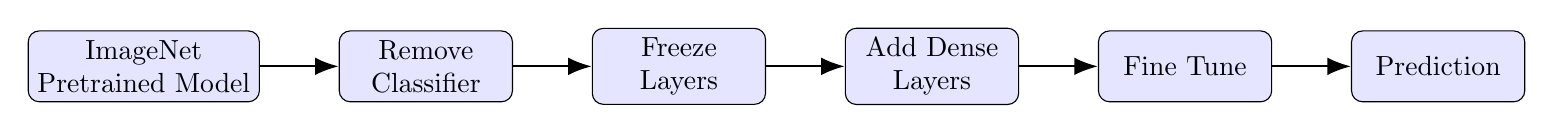
\begin{tikzpicture}[node distance=1cm]

\node[layer](a){ImageNet\\Pretrained Model};

\node[layer,right=of a](b){Remove\\Classifier};

\node[layer,right=of b](c){Freeze\\Layers};

\node[layer,right=of c](d){Add Dense\\Layers};

\node[layer,right=of d](e){Fine Tune};

\node[layer,right=of e](f){Prediction};

\foreach \x/\y in {a/b,b/c,c/d,d/e,e/f}
\draw[arrow](\x)--(\y);

\end{tikzpicture}

\caption{Transfer Learning Workflow}

\end{figure}

Advantages

\begin{itemize}
\item Faster convergence.
\item Higher accuracy on small datasets.
\item Reduced training time.
\item Lower computational cost.
\end{itemize}

%%%%%%%%%%%%%%%%%%%%%%%%%%%%%%%%%%%%%%%%%%%%%%%%%%%%%%%%%%%%

\section*{14. Dataset}

Dataset: CIFAR-10

\begin{itemize}

\item Training Images : 50,000

\item Testing Images : 10,000

\item Number of Classes : 10

\item Image Size : $32\times32\times3$

\item Classes:
Airplane, Automobile, Bird, Cat, Deer,
Dog, Frog, Horse, Ship and Truck.

\end{itemize}

For this experiment the 50,000 training images were further split into a
training set and a validation set (90:10) using a fixed random seed
(\texttt{SEED = 42}) for reproducibility. The actual split obtained was

\begin{itemize}
\item Training set : 45,000 images, shape $(45000,32,32,3)$
\item Validation set : 5,000 images, shape $(5000,32,32,3)$
\item Testing set : 10,000 images, shape $(10000,32,32,3)$
\item Pixel value range after normalization : $[0.000,\,1.000]$
\end{itemize}

%%%%%%%%%%%%%%%%%%%%%%%%%%%%%%%%%%%%%%%%%%%%%%%%%%%%%%%%%%%%
% Continue with Part 3
%%%%%%%%%%%%%%%%%%%%%%%%%%%%%%%%%%%%%%%%%%%%%%%%%%%%%%%%%%%%

\section*{15. Experimental Procedure}

\subsection*{Task 1: Dataset Preparation}

\begin{enumerate}

\item Load the CIFAR-10 dataset using TensorFlow/Keras.

\item Normalize the pixel values to the range [0,1].

\item Display ten sample images.

\item Print the dimensions of the training and testing datasets.

\end{enumerate}

\begin{figure}[H]
\centering
\includegraphics[width=0.95\textwidth]{figs/fig_sample_images.png}
\end{figure}

\textit{Inference:} The sample images confirm that the CIFAR-10 images are
low resolution ($32\times32$) colour photographs with considerable
variation in pose, background and lighting, which makes the classification
task non-trivial even though only 10 classes are involved.

%%%%%%%%%%%%%%%%%%%%%%%%%%%%%%%%%%%%%%%%%%%%%%%%%%%%%%%%%%%%

\subsection*{Task 2: Transfer Learning}

Load any one of the following pretrained CNN models.

\begin{itemize}

\item VGG16

\item ResNet50

\item MobileNetV2

\item EfficientNetB0 (Optional)

\end{itemize}

Perform the following steps.

\begin{enumerate}

\item Load pretrained ImageNet weights.

\item Remove the original classification layer.

\item Freeze the convolutional base.

\item Add a Global Average Pooling layer.

\item Add a Dense layer with ReLU activation.

\item Add the output layer with Softmax activation.

\end{enumerate}

In this implementation \textbf{VGG16} and \textbf{ResNet50} were both
loaded with ImageNet weights (\texttt{include\_top=False}), their
convolutional bases frozen, and the same classification head attached:
Global Average Pooling $\rightarrow$ Dense(ReLU) $\rightarrow$
Dropout(0.3) $\rightarrow$ Dense(10, Softmax). CIFAR-10 images were
resized from $32\times32$ to $96\times96$ before being passed through the
backbone-specific \texttt{preprocess\_input} function. The VGG16
transfer-learning model summary reported

\begin{itemize}
\item Total parameters : 14,848,586 (56.64\ MB)
\item Trainable parameters (frozen stage) : 133,898 (523.04\ KB)
\item Non-trainable parameters (frozen stage) : 14,714,688 (56.13\ MB)
\end{itemize}

%%%%%%%%%%%%%%%%%%%%%%%%%%%%%%%%%%%%%%%%%%%%%%%%%%%%%%%%%%%%

\subsection*{Task 3: Model Training}

Train the model using

\begin{center}

\begin{tabular}{|p{5cm}|p{6cm}|}

\hline

Optimizer & Adam\\

\hline

Learning Rate & 0.001\\

\hline

Batch Size & 32\\

\hline

Epochs & 10--20\\

\hline

Loss Function &
Categorical Cross Entropy\\

\hline

Evaluation Metric &
Accuracy\\

\hline

\end{tabular}

\end{center}

\subsection*{Implementation Details (Actual Configuration Used)}

The experiment was executed on TensorFlow 2.20.0 with two GPUs (Tesla T4)
available and mixed-precision training enabled
(\texttt{mixed\_float16}). The random seed was fixed to 42 for NumPy,
Python and TensorFlow. The exact configuration dictionary used is
summarised below.

\begin{center}
\begin{tabular}{|l|c|}
\hline
Parameter & Value\\
\hline
Number of Classes & 10\\
Validation Split & 0.1\\
Transfer-Learning Image Size & $96\times96$\\
Baseline (from-scratch) Image Size & $32\times32$\\
Batch Size & 64\\
Epochs -- Baseline Models & 12\\
Epochs -- Frozen (Task 3) & 8\\
Epochs -- Fine-Tuning (Task 4) & 6\\
Learning Rate -- Frozen Stage & 0.001\\
Learning Rate -- Fine-Tuning Stage & $1\times10^{-5}$\\
Epochs -- Optimizer Comparison & 5\\
Epochs -- Hyperparameter Search & 4\\
Loss Function & Sparse Categorical Cross-Entropy\\
\hline
\end{tabular}
\end{center}

Three CNNs were also trained \textbf{from scratch} (without transfer
learning) on the native $32\times32$ CIFAR-10 images as baselines for
comparison: a classic \textbf{LeNet-5}, a scaled-down \textbf{AlexNet
(AlexNetMini)} and a scaled-down \textbf{ResNet (ResNetMini)} with a
single residual block. All three baselines and the transfer-learning
frozen stage were trained with the Adam optimizer.

%%%%%%%%%%%%%%%%%%%%%%%%%%%%%%%%%%%%%%%%%%%%%%%%%%%%%%%%%%%%

\subsection*{Task 4: Fine Tuning}

\begin{enumerate}

\item Unfreeze the last convolution block.

\item Train for another 5--10 epochs.

\item Compare the classification accuracy before and after fine tuning.

\end{enumerate}

For VGG16, the last 6 layers of the convolutional base (approximately the
last convolution block) were unfrozen and trained for 6 further epochs
with a reduced learning rate of $1\times10^{-5}$. For ResNet50, the last
10 layers of the convolutional base were unfrozen and trained for 6
further epochs with the same reduced learning rate.

\begin{center}
\begin{tabular}{|l|c|c|}
\hline
Model & Accuracy Before Fine-Tuning & Accuracy After Fine-Tuning\\
\hline
VGG16 & 83.10\% & 90.26\%\\
ResNet50 & 84.41\% & 86.14\%\\
\hline
\end{tabular}
\end{center}

\textit{Inference:} Fine-tuning the last convolution block improved test
accuracy for both backbones. The improvement was much larger for VGG16
(+7.16 percentage points) than for ResNet50 (+1.73 percentage points),
suggesting that VGG16's ImageNet features benefited more from adapting to
the low-resolution CIFAR-10 domain, while ResNet50's residual features
were already closer to optimal for this task even in the frozen state.

%%%%%%%%%%%%%%%%%%%%%%%%%%%%%%%%%%%%%%%%%%%%%%%%%%%%%%%%%%%%

\subsection*{Task 5: Model Evaluation}

Evaluate the trained model using

\begin{itemize}

\item Accuracy

\item Precision

\item Recall

\item F1-score

\item Confusion Matrix

\item Classification Report

\end{itemize}

All models were evaluated on the held-out 10,000-image CIFAR-10 test set
using \texttt{accuracy\_score}, \texttt{precision\_score},
\texttt{recall\_score}, \texttt{f1\_score} (weighted average),
\texttt{confusion\_matrix} and \texttt{classification\_report} from
scikit-learn. The detailed results are reported in Section 18.

%%%%%%%%%%%%%%%%%%%%%%%%%%%%%%%%%%%%%%%%%%%%%%%%%%%%%%%%%%%%

\section*{16. Hyperparameter Study}

Compare the performance using different settings.

\begin{center}

\begin{tabular}{|l|l|}

\hline

Hyperparameter & Values\\

\hline

Learning Rate &
0.001, 0.0001\\

\hline

Batch Size &
16, 32, 64\\

\hline

Epochs &
10, 20\\

\hline

Optimizer &
Adam, SGD\\

\hline

Dense Units &
128, 256\\

\hline

Frozen Layers &
All, Partial\\

\hline

\end{tabular}

\end{center}

\subsection*{16.1 Optimizer Comparison (VGG16, 5 epochs, $96\times96$ input)}

\begin{center}
\begin{tabular}{|l|c|c|c|}
\hline
Optimizer & Test Accuracy (\%) & F1-score & Training Time (s)\\
\hline
Adam (lr = 0.001) & 82.79 & 0.8278 & 89.0\\
SGD (lr = 0.01, momentum = 0.9) & 80.79 & 0.8079 & 88.1\\
\hline
\end{tabular}
\end{center}

\begin{figure}[H]
\centering
\includegraphics[width=0.95\textwidth]{figs/fig_adam_vs_sgd_curves.png}
\end{figure}

\textit{Inference:} Adam converged faster and reached a lower validation
loss and higher validation accuracy than SGD within the same epochs.

\subsection*{16.2 Hyperparameter Search Results (VGG16, 4 epochs each)}

\begin{center}
\begin{tabular}{|c|c|l|c|c|}
\hline
Learning Rate & Dense Units & Frozen Layers & Validation Accuracy & Time (s)\\
\hline
0.0010 & 128 & All & 0.8330 & 73.4\\
0.0010 & 256 & All & 0.8402 & 72.8\\
0.0001 & 256 & Partial (last 4 layers unfrozen) & 0.9098 & 89.0\\
\hline
\end{tabular}
\end{center}

\textit{Inference:} Increasing the dense layer width from 128 to 256
units gave a small improvement in validation accuracy (+0.72 points) at
almost no extra time cost. Partially unfreezing the convolutional base
combined with a lower learning rate gave the largest gain
(+6.96 points over the best fully-frozen configuration), confirming that
allowing some backbone layers to adapt to CIFAR-10 is more valuable than
simply widening the classifier head.

%%%%%%%%%%%%%%%%%%%%%%%%%%%%%%%%%%%%%%%%%%%%%%%%%%%%%%%%%%%%

\section*{17. Mandatory Plots}

Include the following plots in the laboratory report.

\begin{enumerate}

\item Sample CIFAR-10 images

\item Training Accuracy

\item Validation Accuracy

\item Training Loss

\item Validation Loss

\item Confusion Matrix

\item Misclassified Images (Optional)

\end{enumerate}

Students should write a brief inference (2--3 lines) for each figure.

\subsection*{17.1 Baseline (From-Scratch) Models}

\begin{figure}[H]
\centering
\includegraphics[width=0.95\textwidth]{figs/fig_lenet5_curves.png}
\end{figure}

\textit{Inference:} LeNet-5's training and validation accuracy increase
slowly and converges across iterations, with no overfitting, but the
final accuracy plateaus around 54\%, reflecting the model's lower capacity.

\begin{figure}[H]
\centering
\includegraphics[width=0.7\textwidth]{figs/fig_lenet5_cm.png}
\end{figure}

\textit{Inference:} LeNet-5 could not classify visually similar classes such as
cat/dog and automobile/truck, but performs relatively well on
more distinctive classes such as ship and automobile.

\begin{figure}[H]
\centering
\includegraphics[width=0.95\textwidth]{figs/fig_alexnet_curves.png}
\end{figure}

\textit{Inference:} AlexNetMini shows a steady increase in
accuracy and decrease in loss, reaching around 75\% training and
validation accuracy by epoch 12, indicating good generalisation.

\begin{figure}[H]
\centering
\includegraphics[width=0.7\textwidth]{figs/fig_alexnet_cm.png}
\end{figure}

\textit{Inference:} AlexNetMini achieves good classification across
most classes, with the main confusion remaining between cat, dog and bird,
which have lesser distinctive feature.

\begin{figure}[H]
\centering
\includegraphics[width=0.95\textwidth]{figs/fig_resnetmini_curves.png}
\end{figure}

\textit{Inference:} Training for ResNetMini was stopped early once validation loss
stopped improving; the restored weights generalised
poorly to the test set (47.26\% accuracy), suggesting the small residual
model was not strong enough to be trained stably in so few
epochs.

\begin{figure}[H]
\centering
\includegraphics[width=0.7\textwidth]{figs/fig_resnetmini_cm.png}
\end{figure}

\textit{Inference:} ResNetMini's confusion matrix shows heavy bias toward
a few classes, with the truck class predicted poorly, proving the unstable,
under-trained behaviour.

\subsection*{17.2 Transfer Learning -- VGG16}

\begin{figure}[H]
\centering
\includegraphics[width=0.95\textwidth]{figs/fig_vgg_frozen_curves.png}
\end{figure}

\textit{Inference:} With the convolutional base frozen, VGG16 already
reaches roughly 84--86\% training accuracy and 83--84\% validation
accuracy within 8 epochs.

\begin{figure}[H]
\centering
\includegraphics[width=0.7\textwidth]{figs/fig_vgg_frozen_cm.png}
\end{figure}

\textit{Inference:} The frozen VGG16 model is strong across nearly all
classes, with the largest remaining confusion between cat and dog.

\begin{figure}[H]
\centering
\includegraphics[width=0.95\textwidth]{figs/fig_vgg_ft_curves.png}
\end{figure}

\textit{Inference:} After unfreezing the last convolution block, training
accuracy increases to 96\% while validation accuracy reaches about
91\%, indicating mild overfitting.

\begin{figure}[H]
\centering
\includegraphics[width=0.7\textwidth]{figs/fig_vgg_ft_cm.png}
\end{figure}

\textit{Inference:} Fine-tuning sharpens the diagonal of the confusion
matrix considerably compared to the frozen model, especially for
automobile, ship and truck, which now exceed 90\% recall.

\begin{figure}[H]
\centering
\includegraphics[width=0.95\textwidth]{figs/fig_vgg_misclassified.png}
\end{figure}


\subsection*{17.3 Transfer Learning -- ResNet50}

\begin{figure}[H]
\centering
\includegraphics[width=0.95\textwidth]{figs/fig_resnet50_frozen_curves.png}
\end{figure}

\textit{Inference:} ResNet50's frozen backbone converges faster than
VGG16's, reaching about 86-87\% validation accuracy within just 4 epochs, proving that ResNet 50 is better than VGG16.

\begin{figure}[H]
\centering
\includegraphics[width=0.7\textwidth]{figs/fig_resnet50_frozen_cm.png}
\end{figure}

\textit{Inference:} The frozen ResNet50 model gives a
confusion matrix with high recall across most classes; cat and dog remain
the most confused pair.

\begin{figure}[H]
\centering
\includegraphics[width=0.95\textwidth]{figs/fig_resnet50_ft_curves.png}
\end{figure}

\textit{Inference:} Fine-tuning the last 10 layers of ResNet50 gives a
minimal additional gain than for VGG16, as the training and validation
curves rise only little beyond the frozen-stage result, suggesting
ResNet50's frozen features were already close to their maximum performance.

\begin{figure}[H]
\centering
\includegraphics[width=0.7\textwidth]{figs/fig_resnet50_ft_cm.png}
\end{figure}

\textit{Inference:} Fine-tuning improves ResNet50's precision and recall
slightly across almost every class compared to the frozen model, with the
largest gains for the cat and dog classes.

\subsection*{17.4 Overall Comparison}

\begin{figure}[H]
\centering
\includegraphics[width=0.75\textwidth]{figs/fig_frozen_vs_finetuned_bar.png}
\end{figure}

\textit{Inference:} Fine-tuning improves test accuracy for both
backbones, VGG16 gains substantially
from fine-tuning and overtakes ResNet50,
whereas ResNet50's frozen accuracy was already higher than VGG16's and it
gains comparatively little from fine-tuning.

%%%%%%%%%%%%%%%%%%%%%%%%%%%%%%%%%%%%%%%%%%%%%%%%%%%%%%%%%%%%

\section*{18. Results}

\subsection*{18.1 Performance Metrics (Best Model: VGG16, Fine-Tuned)}

\begin{center}

\begin{tabular}{|p{5cm}|p{4cm}|}

\hline

Metric & Value\\

\hline

Training Accuracy & 96.39\%\\

\hline

Testing Accuracy & 90.26\%\\

\hline

Precision & 0.9035\\

\hline

Recall & 0.9026\\

\hline

F1-score & 0.9028\\

\hline

Training Time & 290.3 s (fine-tuning stage; 141.1 s frozen stage)\\

\hline

Total Parameters & 14,848,586\\

\hline

\end{tabular}

\end{center}

\vspace{5mm}

\subsection*{18.2 Comparison of CNN Architectures (Experimental Results)}

\begin{center}

\begin{tabular}{|l|c|c|c|c|c|c|}

\hline

Model &
Parameters &
Test Accuracy (\%) &
Precision &
Recall &
F1-score &
Training Time (s)\\

\hline

LeNet-5  & 83{,}126 & 54.26 & 0.5481 & 0.5426 & 0.5403 & 232.8\\

\hline

AlexNetMini & 6{,}976{,}842 & 75.26 & 0.7575 & 0.7526 & 0.7486 & 306.1\\

\hline

ResNetMini & 681{,}226 & 47.26 & 0.5552 & 0.4726 & 0.4317 & 141.1\\

\hline

VGG16 (Frozen, TL) & 14{,}848{,}586 & 83.10 & 0.8323 & 0.8310 & 0.8306 & 141.1\\

\hline

VGG16 (Fine-Tuned, TL) & 14{,}848{,}586 & 90.26 & 0.9035 & 0.9026 & 0.9028 & 290.3\\

\hline

ResNet50 (Frozen, TL) & -- & 84.41 & 0.8455 & 0.8441 & 0.8440 & 91.1\\

\hline

ResNet50 (Fine-Tuned, TL) & -- & 86.14 & 0.8614 & 0.8614 & 0.8613 & 194.3\\

\hline

\end{tabular}

\end{center}

%%%%%%%%%%%%%%%%%%%%%%%%%%%%%%%%%%%%%%%%%%%%%%%%%%%%%%%%%%%%

\section*{19. Discussion Questions}

Answer the following questions.

\begin{enumerate}

\item Why is AlexNet considered a breakthrough in deep learning?\\
AlexNet was considered a major breakthrough in Deep Learning, as it introduced the usage of ReLU activation function, introduction of dropouts, data augmentation, multiple CNN layers and parallel GPU training. These features of AlexNet improved the performance led to faster convergence, with a higher accuracy.

\item Why does VGG16 use only $3\times3$ convolution filters?\\
VGG Net uses 3x3 filter because, it is proved efficient than larger filters by reducing the parameter size and using multiple 3x3 filter also increases the receptive field. VGG16 achieved good feature extraction using the 3x3 filter, proving its efficiency over larger filters.

\item Explain the advantages of the Inception module.\\
Inception module simultaneously uses multiple filters of different sizes, trains the model and is stacked together. The usage of 1x1 filter produces feature map that contains the most important feature. Thus Inception Module, provides a better feature extraction, pooling and better feature maps, keeping the computation less intensive.

\item What is the purpose of residual learning?\\
Residual Learning aids in skipping the connections that are not relevant for the training. It allows gradients to flow directly through shortcut connections, thereby reducing the vanishing gradient problem.

\item Differentiate LeNet and ResNet.\\
LeNet is a primitive early stage CNN Network that has a shallow network with fewer layers. It works using convolution technique and pooling. On the other hand, ResNet is a much deeper architecture designed to train efficiently using residual connections. It has a deeper network with multiple layers, helping for large scale image recognition tasks. It uses skip connection which a key aspect of ResNet.

\item What is Transfer Learning?\\
Transfer Learning is a technique where a model trained on one task is reused for another related task. Instead of training a model from scratch, the pretrained model's learned features are reused. It reduces the training time at the same time provides a better accuracy.

\item Why is fine tuning required?\\
Fine-tuning is required because a pretrained model was originally trained for a different task. Fine-tuning helps in improving the accuracy for a task on top of the baseline accuracy while retaining the knowledge of pretrained model.

\item Explain the difference between dilated convolution and transpose convolution.\\
A dilated convolution inserts spaces between kernel elements. It increases the receptive field without increasing the number of parameters. Transpose convolution, on the other hand, increases the spatial dimensions of feature maps.

\item Why do pretrained models converge faster?\\
Pretrained models converges faster because they already have useful parameters learned from the previous dataset. Within a fewer epochs, a higher accuracy could be achieved due the prior knowledge of the task.

\item Compare the computational complexity of LeNet and ResNet.\\
LeNet is computationally less intensive as it has fewer layers and lesser parameters. ResNet on the other hand, contains many layers, has multiple convolutional blocks, and uses for processing huge dataset. Thus ResNet is computationally more intensive.
\end{enumerate}

%%%%%%%%%%%%%%%%%%%%%%%%%%%%%%%%%%%%%%%%%%%%%%%%%%%%%%%%%%%%

\section*{20. Additional Exercises}

\begin{enumerate}

\item Implement transfer learning using VGG16.

\item Repeat the experiment using ResNet50.

\item Compare Adam and SGD optimizers.

\item Compare training with frozen layers and fine tuning.

\item Evaluate the model using Precision, Recall and F1-score.

\item Compare the performance of LeNet, AlexNet and ResNet.

\end{enumerate}

%%%%%%%%%%%%%%%%%%%%%%%%%%%%%%%%%%%%%%%%%%%%%%%%%%%%%%%%%%%%

\section*{21. References}

\begin{enumerate}

\item Yann LeCun, Leon Bottou, Yoshua Bengio and Patrick Haffner,
\emph{Gradient-Based Learning Applied to Document Recognition},
Proceedings of the IEEE, 1998.

\item Alex Krizhevsky, Ilya Sutskever and Geoffrey Hinton,
\emph{ImageNet Classification with Deep Convolutional Neural Networks},
NeurIPS, 2012.

\item Karen Simonyan and Andrew Zisserman,
\emph{Very Deep Convolutional Networks for Large-Scale Image Recognition},
ICLR, 2015.

\item Christian Szegedy et al.,
\emph{Going Deeper with Convolutions},
CVPR, 2015.

\item Kaiming He, Xiangyu Zhang, Shaoqing Ren and Jian Sun,
\emph{Deep Residual Learning for Image Recognition},
CVPR, 2016.

\item Ian Goodfellow, Yoshua Bengio and Aaron Courville,
\emph{Deep Learning},
MIT Press, 2016.

\item TensorFlow Documentation:
\url{https://www.tensorflow.org}

\item Keras Documentation:
\url{https://keras.io}

\end{enumerate}

%%%%%%%%%%%%%%%%%%%%%%%%%%%%%%%%%%%%%%%%%%%%%%%%%%%%%%%%%%%%

\end{document}
